\title{MINIPROJECT\\
3D OBJECT SCANNER}
\author{
        Department of Electronics And Communication\\
       Model Engineering College\\
       Thrikkakara\\
       \\
       TEAM MEMBERS:\\
        1.KIRAN S KURIAN\\
        2.GAUTHAM M        \\
        3.ANNE KALLOOR RAJU\\
        4.SUKANYA SASIKUMAR\\
        5.SHAMEEM PARAPPORU\\
}
%\date{}

\documentclass[12pt,a4paper,oneside]{report}


\usepackage{amsfonts}
\usepackage{textcomp}
\usepackage{graphicx}
\usepackage{setspace}
\usepackage{fancyhdr}
\usepackage{truncate}
\usepackage{nomencl} 
\usepackage{array}
\usepackage{caption}
\usepackage{subcaption}
\usepackage{subfig}
\usepackage[overload]{textcase}
\renewcommand{\nomname}{List of Abbreviations}
\makenomenclature



\usepackage{titlesec}
\titleformat{\chapter}[display]
  {\normalfont\Large\bfseries\centering}
 {\chaptertitlename\ \thechapter}{20pt}{\LARGE}
\titleformat{\section}{\large\bfseries}{\thesection}{1em}{}
\titleformat{\subsection}{\normalsize\bfseries}{\thesubsection}{1em}{}



\renewcommand{\chaptermark}[1]{\markboth{ \emph{#1}}{}}

\begin{document}
\maketitle
\thispagestyle{empty}

\pagenumbering{roman}



\begin{onehalfspacing}


\chapter{\uppercase{INITIAL REPORT}}

\pagenumbering{arabic}



\section{BLOCK DIAGRAM DESCRIPTION}



{$\;\;\;\;$}
A 3D scanner is a device that analyses a real-world object or environment to collect data on its shape and possibly its appearance. The collected data can then be used to construct digital, three dimensional models. Fig 2.1 is the block diagram of the 3D scanner.

\begin{figure}[htb]
\begin{center}
\leavevmode
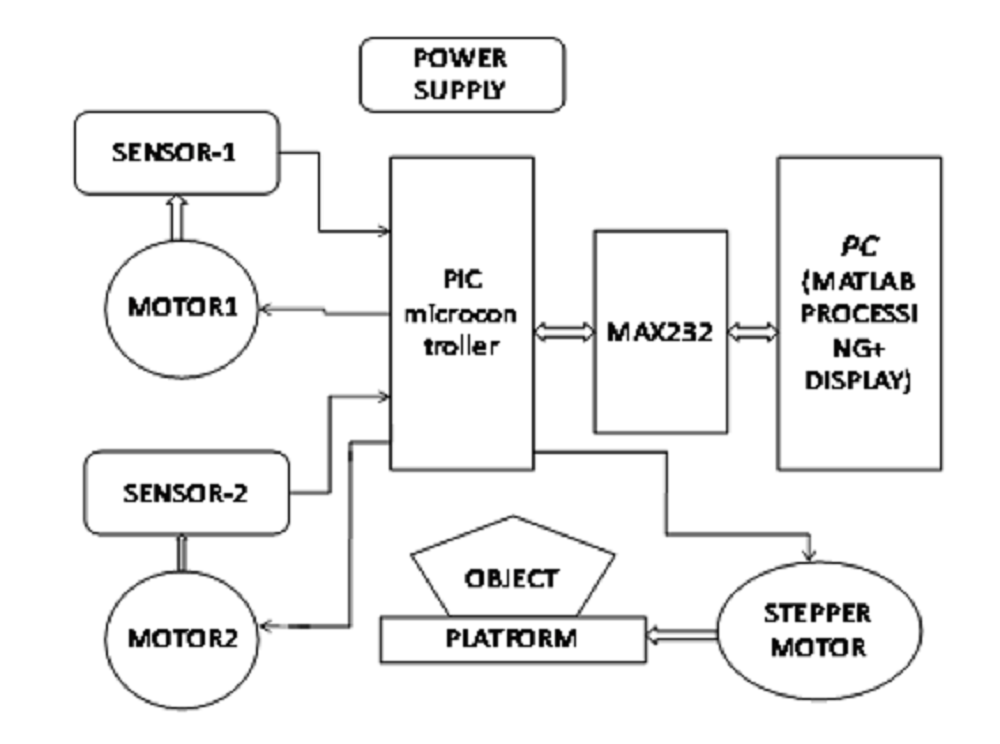
\includegraphics[width=0.25\textwidth]{fig01.png}
\end{center}
\caption[Block Diagram]{\emph{Block Diagram}$^{ \scriptsize {\cite{r4}}}$}
\label{fig1}
\end{figure}

\section{CIRCUIT DIAGRAM}
{$\;\;\;\;$}

\begin{figure}[htb]
\begin{center}
\leavevmode
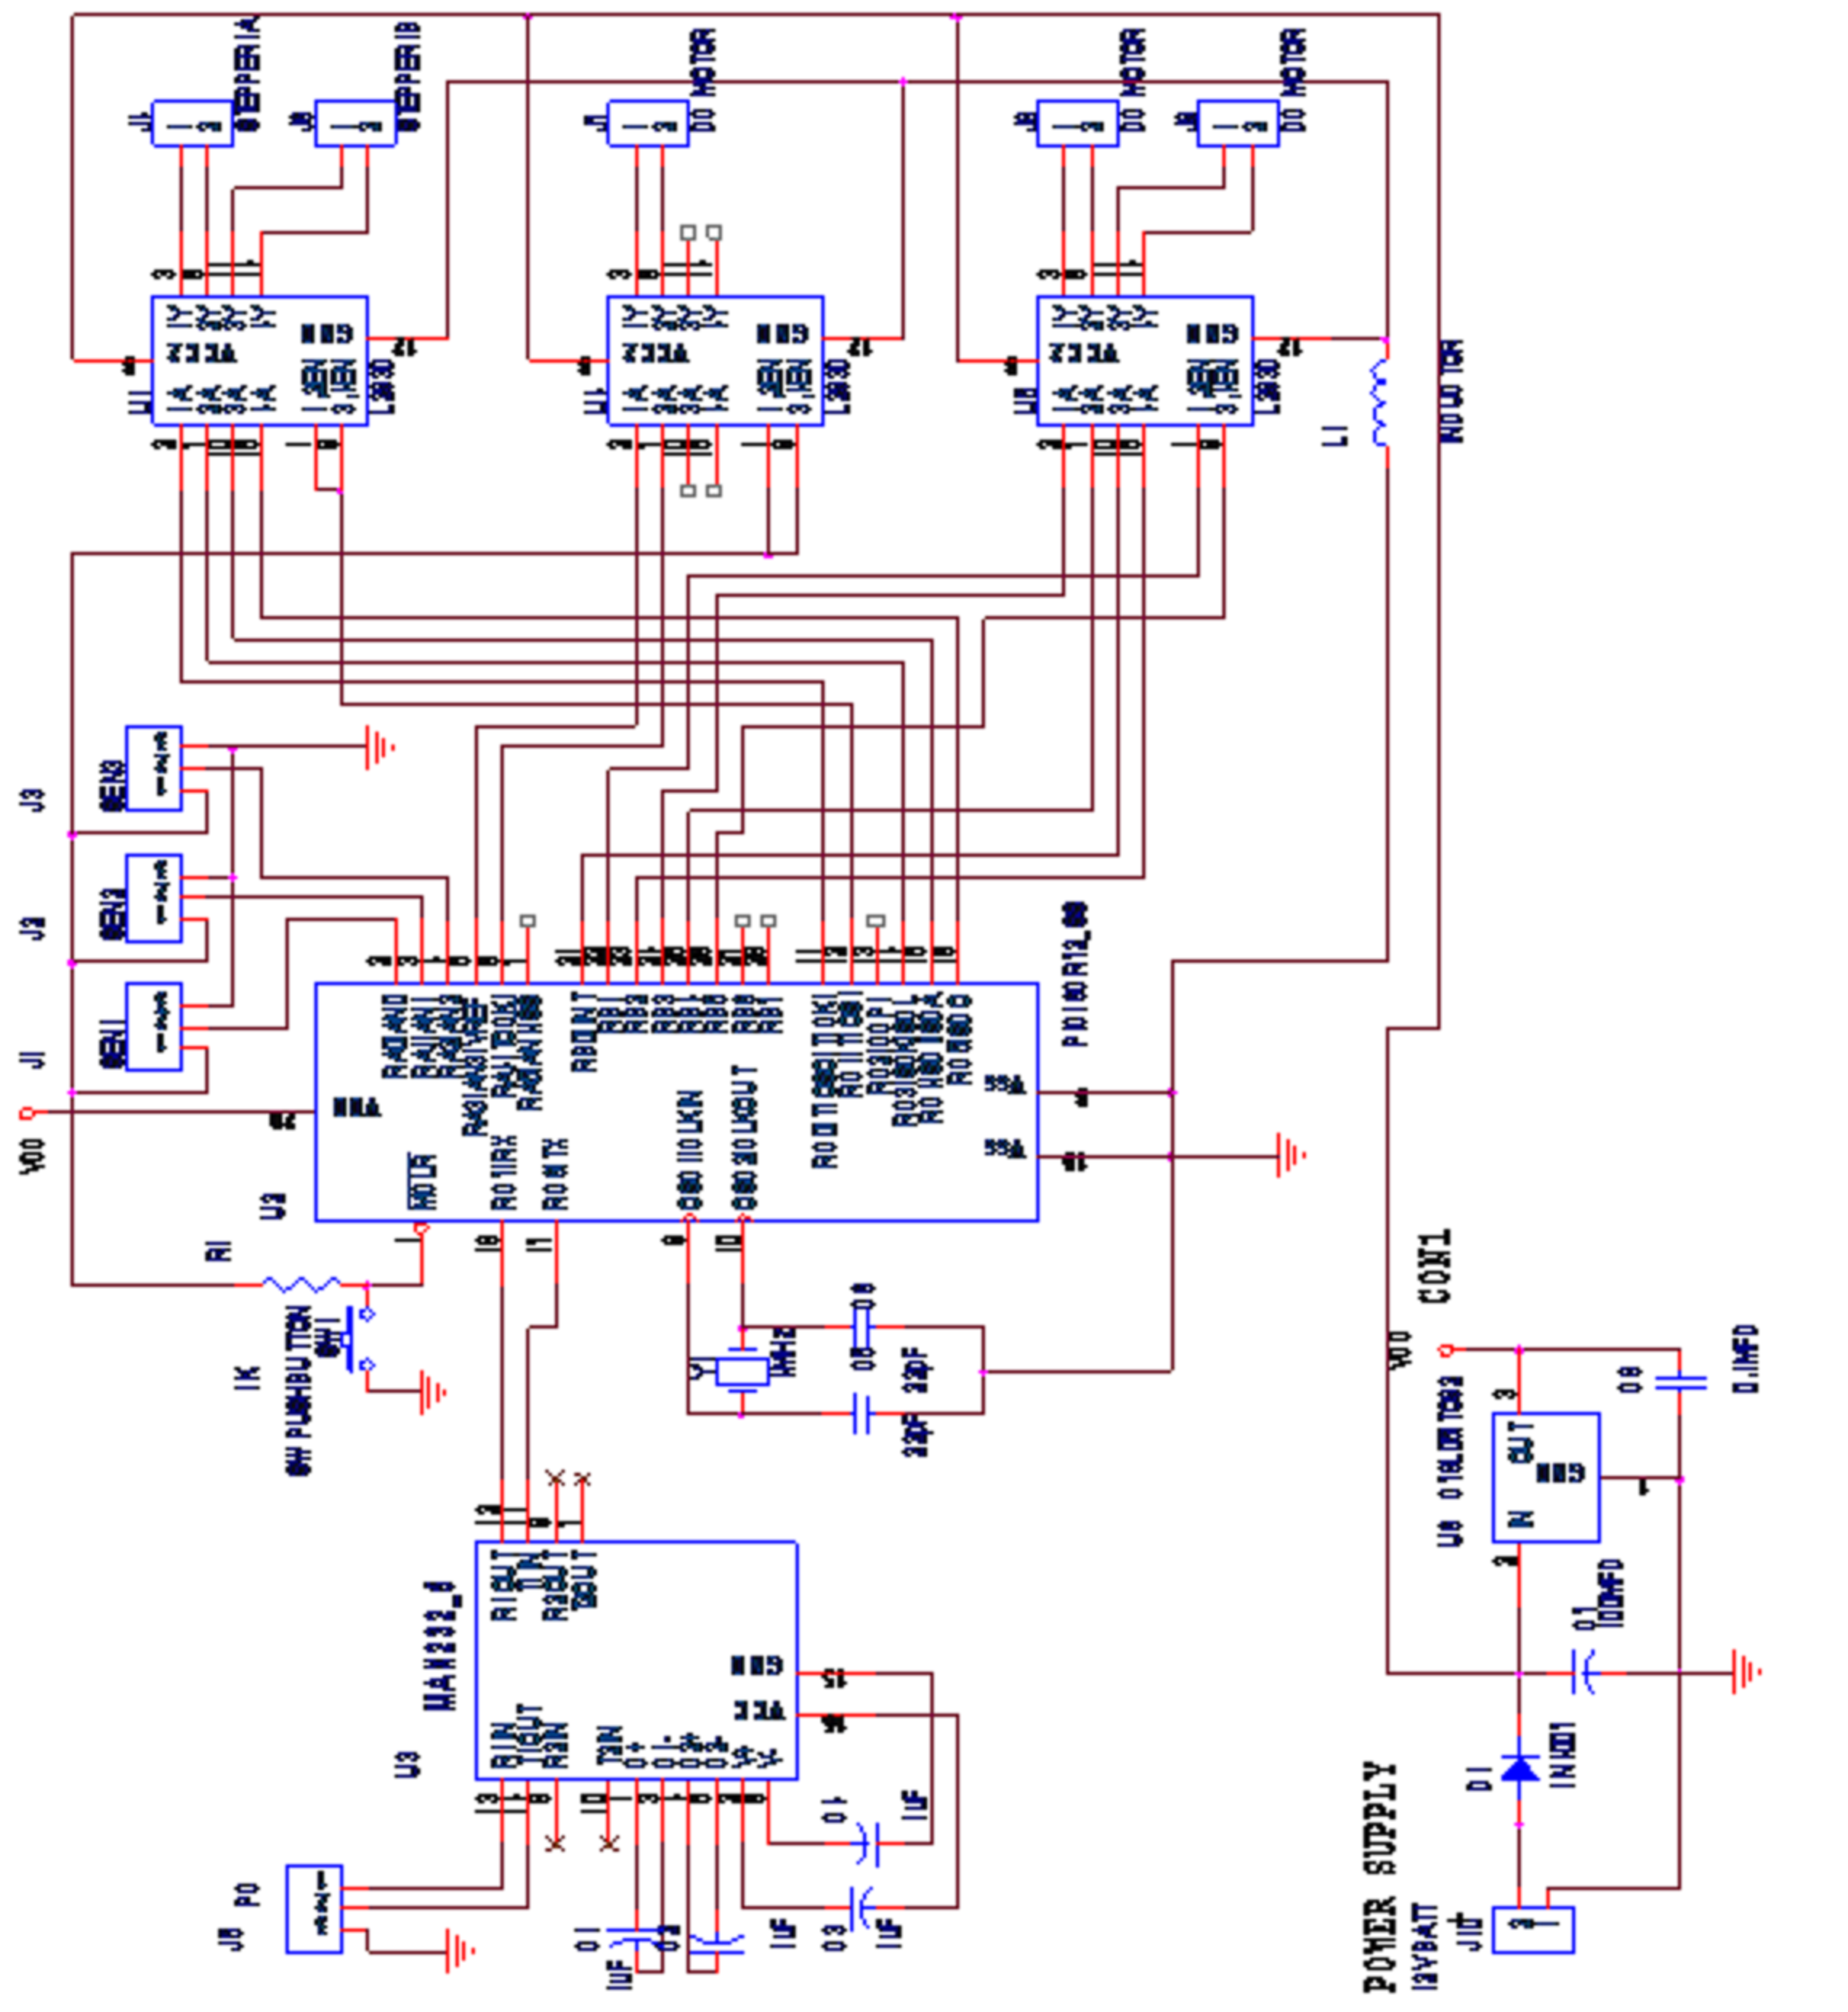
\includegraphics[width=0.25\textwidth]{fig02.png}
\end{center}
\caption[Circuit Diagram]{\emph{Circuit Diagram}$^{ \scriptsize {\cite{r4}}}$}
\label{fig1}
\end{figure}



\section{CIRCUIT WORKING}
\par
\hspace{.7cm}
Fig   is the circuit diagram of the 3D Object Scanner. The supply to the circuit is provided by an LM7805 IC. It consists of a PIC microcontroller.The PIC used here is PIC 16F883.It is the control unit for the entire system.L293D motor drivers are connected to the analog input pins of the PIC. These motor drivers are used to rotate the stepper and DC motors used to rotate the turn table and the sensors. The IR Proximity sensors are used to detect the object and to measure its coordinate distances. These are also connected to the analog input pins.A MAX 232 IC is connected to the transmit and receive pins of the PIC for its communication with the PC.
\par
When the power is on, all the circuit elements get the required supply voltage of +5 volt. Then the enable pins of motor driver get a high voltage and thus the motor drivers are enabled and will provide a bidirectional drive current. This drives the motors connected to the driver IC. As the motor starts rotating, the turn table and the sensors start their movement. Then the IR sensors start to detect the object and will send the distance information to the PIC. The PIC stores this distance information and sends this to a PC using a MAX 232 IC. 

\chapter{\uppercase{MECHANICAL STRUCTURE}}
{$\;\;\;\;$}The fig   shows the mechanical structure of the 3D object scanner. It consists of a turn table, distance sensors, motors, and threaded vertical rod. The object to be scanned is placed on the turn table. A motor is connected to the turn table. The distance sensors are attached to a threaded vertical rod. A motor is also connected to the threaded vertical rod
\par
The turn table is then rotated using the motor connected to it. It is rotated at angle of 360 degrees. The distance sensors connected to the threaded vertical rod measures the co-ordinate values of the object to be scanned. After completing the first round of rotation, the distance sensors are moved vertically and again the co-ordinates are measured. This process continues until the top of the object is scanned. 

\section{REFERENCES}
{$\;\;\;\;$}
\begin{enumerate}	
\item [1]. Borghese N A, “Auto scan, a flexible and portable 3D scanner” 1998  IEEE.
\item [2]. Jin Sun, “Triangular mesh generation for a real structure scan data in 3D space” 2011 IEEE.
\item [3].Ohno and Kazunori, “3D Scanner for measuring uniform and dense 3D shapes of static objects”2008 IEEE.
\item [4]. Roennau A, “Robust 3D scan segmentation for tele operation task in areas contaminated by radiation” 2010 IEEE.
\item [5]. Xiaozhi Li, “Human body dimensions extraction from 3D scan data” 2010 IEEE.
\end{enumerate}


\section{FEASIBILITY REPORT}
{$\;\;\;\;$}	
\begin{itemize}
\item MOTORS                             : Rs. 500
\item BATTERY                            : Rs. 500
\item PIC16F883(MICROCONTROLLER)         : Rs. 100
\item IR PROXIMITY SENESOR(GP2Y0A21YK)   : Rs. 1500
\item DB9 CONNECTOR                      : Rs. 15
\item L293D(MOTOR DRIVE IC)              : Rs. 220
\item MAX232(IC)                         : Rs. 30
\item IC HOLDERS                         : Rs. 10
\item CIRCUIT BOARD FABRICATION          : Rs. 300
\item MISCELANEOUS EXPENSES              : Rs. 100
\item RESERVE                            : Rs. 500
\item TOTAL                              : Rs. 3775
\end{itemize}

\end{onehalfspacing}
\end{document}
